\chapter{Simulating GOTO Observations}
\label{chap:sims}
\chaptoc{}

% ########################################

\newpage
\section{Introduction}
\label{sec:sims_intro}
\begin{colsection}

% ~~~~~~~~~~~~~~~~~~~~

\begin{colsection}

In this chapter I outline my work creating simulations of the GOTO observatory. Section~\ref{sec:scheduler_sims} describes simulations carried out in order to find the optimal ``tie-break'' parameters for the \gls{gtecs} scheduler, while Section~\ref{sec:multitel_sims} describes simulations of the combined response of multiple GOTO telescopes observing gravitational wave skymaps and the all-sky survey. All work described in this chapter is my own and has not been published before anywhere else.

\end{colsection}

% ~~~~~~~~~~~~~~~~~~~~

\subsection{Simulating GOTO}
\label{sec:goto_sims}
\begin{colsection}

WIP

\end{colsection}

% ~~~~~~~~~~~~~~~~~~~~

\end{colsection}

% ########################################

\newpage
\section{Scheduler simulations}
\label{sec:scheduler_sims}
\begin{colsection}

% ~~~~~~~~~~~~~~~~~~~~

\begin{colsection}

The scheduler is described in in Section~\ref{sec:scheduler}.

Why do we need a tie-break? (described previously a bit, but worth reminding)

The different tie-break parameters:
\begin{itemize}
    \item Airmass, obviously
    \item Weight, also obviously
    \item Time to set / time valid?
\end{itemize}

Simulations

Output: plot airmass vs time observed

\rtxt{still work to do}

\end{colsection}

% ~~~~~~~~~~~~~~~~~~~~
\end{colsection}

% ########################################

\newpage
\section{Multi-telescope and multi-site simulations}
\label{sec:multitel_sims}
\begin{colsection}

% ~~~~~~~~~~~~~~~~~~~~

\begin{colsection}

As described in Section~\ref{sec:goto_expansion}, the ultimate aim of the \gls{goto} project is to have multiple nodes around the world. Specifically, the plan calls for two full GOTO-8 systems on La Palma and another two at a second site in Australia (the exact site is not yet determined, but it will most likely either be either Siding Spring in New South Wales or Mt Kent in Queensland).

In order to better quantify the benefit multiple telescopes and sites will provide, a series of simulations were carried out. These simulations focused on two main areas: the all-sky survey coverage and cadence, and the combined system's response to gravitational wave alerts.

\end{colsection}

% ~~~~~~~~~~~~~~~~~~~~

\subsection{Simulating multiple telescopes and sites}
\label{sec:multi_site}
\begin{colsection}

As outlined in Section~\ref{sec:gtecs_multisite} it is envisioned that, as GOTO expands to multiple telescopes and sites, the \gls{gtecs} scheduling system will be extended so that all the telescopes query a single observation database and a master scheduler decides what each telescope should be observing at a given time. This will require a large amount of work to modify both the database structure and the scheduling functions, and as it is not currently implemented into the existing scheduler several workarounds needed to be used in order to create realistic multi-telescope simulations.

% ---------
\subsubsection{Scheduling for multiple observing telescopes}

One of the current restrictions in the scheduling functions (as described in Section~\ref{sec:scheduler}) is that they only ever expect a single Pointing in the observing database to be marked as \code{running} at any one time. It is explicitly coded into the scheduler that detecting multiple running pointings should raise a critical error, as certain bugs early in development could lead to this undesired state to occur. Obviously once the system is to be expanded to multiple telescopes this restriction will have to be lifted, but for these simulations a simplification was required to work around this restriction.

It is currently planned that each telescope will have its own pilot and hardware daemons completely independent of each other, with the only point of overlap being the shared scheduler (and, most likely, the conditions daemon). This makes the master scheduler even harder to consider, as each pilot will be querying it completely out-of-sync. If telescope 1 has just finished observing and makes a scheduler check the scheduler will need to know what telescope 2 is observing, so as not to return the same pointing to telescope 1 (although in some cases having both telescopes observe the same target might be desired, this adds yet another level of complexity). But should both telescopes finish observing at the same time then the scheduler will need some way to decide which gets what target, perhaps deciding by slew time from each telescope's current position.

As none of the above was implemented into the existing code a simplified system was required for these simulations. The existing fake pilot code (\rtxt{described in the previous section}) already contains calls to the real scheduling functions, which return the highest pointing at given time. The simple modification was to make the function return the top $N$ highest pointings, where $N$ is the number of currently observing telescopes. In lieu of any better algorithm to decide which telescope observes which the code simply gives the highest priority pointing to telescope 1, the second highest to telescope 2 and so on. Should there only be one valid pointing returned then only telescope 1 will observe, while telescope 2 will remain ``parked'' until it is needed (this was relevant for the gravitational wave simulations, in practice the second telescope would default to observing the all-sky survey until it also has something to do).

The second simplification was to ensure the telescopes always stayed in sync when observing. The was doable because for either scenario (all-sky survey or \gls{gw} follow-up) each of the pointing would have identical exposure times and therefore take the same amount of time to observe. As there is no need to include simulation steps while the cameras would be exposing the simulation simply increased the time until the observations would be completed. In practice each telescope would take a different amount of time to slew to its target and so quickly get out of sync. Slew time is included in the fake pilot code, from each telescope to its new target. However in order to remain synchronised the code waits the required amount of time for both telescopes to slew and finish their observations. This also accounts for the multiple-running-pointings issue, as by modifying the simulation steps to skip over the actual observing time the pointings never actually need to be marked as \code{running} in the database --- simply going from \code{pending} to \code{completed}. The real observing database would also need a way to record which pointing was observed by which telescope, but that is stored within the fake pilot so there was no need to modify the database schema.

% ---------
\subsubsection{Scheduling for multiple observing sites}

The above system provides a good approximation of the response of an arbitrary number of telescopes observing at one site. However expanding the code further to simulate observations from multiple sites adds further complexity.

The scheduler needs to know which site observations are being made from, because it takes into account horizon visibility and airmass. That's simple to include if you have only one site observing at once, but once there are telescopes at multiple sites querying the scheduler at the same time then the responses will need to take that into account. For example, with two telescopes at two sites observing at once the scheduler would need to return the top two pointings at each site, as discussed above. However if the visible portions of the sky from both sites overlap then it's very possible that the same pointing could be the highest priority from both sites. The scheduler would have to chose which of the four telescopes to assign that pointing to, most likely based on the airmass at each site or the slew time from the current target. But then the site that didn't get that pointing assigned now only has the one remaining target to share between its two telescopes. In practice this would mean when querying the scheduler it would have to return the top $X$ pointings, where $X = N_\text{site1} + N_\text{site2} + \cdots$ is the total number of telescopes across the globe (for this example $X=4$).

\begin{figure}[t]
\begin{center}
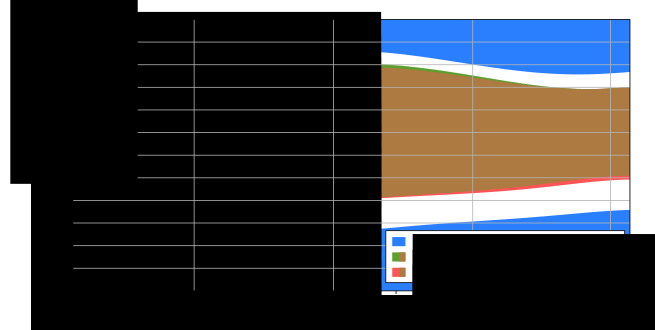
\includegraphics[width=\linewidth]{images/nights.pdf}
\end{center}

\caption[Night times throughout the year for GOTO sites]{Night times throughout the year for GOTO sites. Night here is defined as when the Sun is \SI{12}{\degree} below the local horizon.
}
\label{fig:nights}
\end{figure}

The above system would be possible to implement in the simulations, but there is a lucky simplification that can be made for the specific cases that are being considered. Saying the scheduler needs to find the top $X$ pointings, where $X$ is the total number of telescopes at all sites, is not strictly true --- it actually only needs to return enough pointings to satisfy the telescopes at the sites that are currently observing. In other words it there are two sites but one is shut down, due to weather or because it is daytime there, the scheduler doesn't need to worry about choosing which site pointings are assigned to as only the one is currently active. Conveniently for simulating the proposed GOTO network this is always true: using a horizon of \SI{-12}{\degree} the periods of darkness between La Palma and either of the Australian sites never overlap. This is shown in Figure~\ref{fig:nights}, where there is a constant ``buffer zone'' between night ending at one site and beginning at the other. This case only applies for a very limited number of combinations of sites. As shown in Figure~\ref{fig:site_nights} there is a tear-drop-shaped area on the Earth's surface which contain the locations where the local night will never overlap with night on La Palma, comprising only of eastern Australia, New Zealand and Melanesia. For a horizon of \SI{-12}{\degree} this area contains just $6.6 \%$ of the Earth's surface.

\begin{figure}[p]
\begin{center}
\includegraphics[width=\linewidth]{images/sites.pdf}
\end{center}

\caption[Locations on the Earth with non-overlapping night times]{Finding locations on the Earth with non-overlapping night times. On the upper plot the filled areas show the locations on the Earth where local night never overlaps with night on La Palma, at any point in the year. The different colours denote different horizon definitions, with the \SI{-12}{\degree} horizon also being surrounded by a white dashed line. The location of the GOTO sites considered (\textcolor{blue}{La Palma}, \textcolor{ForestGreen}{Siding Spring} and \textcolor{red}{Mt Kent}) are marked with stars and their antipodes are marked with hollow circles. The equivalent areas for Siding Spring and Mt Kent are also shown by the coloured dashed lines surrounding their antipodes, for a \SI{-12}{\degree} horizon only. The lower plots shows how the region varies over a year, from the solstices via the equinox (the plot is identical for the March and September equinoxes and therefore is only shown once).
}
\label{fig:site_nights}
\end{figure}

\clearpage

The convenient location of the Australian sites means implementing them into the simulation code was fairly simple. Should simulations for other sites on the Earth be included that aren't within the small non-overlapping area, for example other backup GOTO-South sites in South Africa or Chile, the code would need to be expanded as described above. In principle the simulations can be run for any one site on the Earth as a stand-alone observatory, and then this could be combined afterwards with the results from other, stand-alone simulations. This however removes the benefit of the sites acting together and using a common observing database. The method is however used in Section~\ref{sec:gw_sims} below for sites with different grids, where the consequences are examined in more detail.

% ---------
\subsubsection{Simulating different grids}

One fundamental feature of the existing \gls{goto} code is that observations are carried out on an all-sky grid, as defined in Section~\ref{sec:gototile}. When considering multiple telescopes this is both useful in some ways and limiting in others. Having a fixed grid that is common to all telescopes is vital for the \gls{goto} image subtraction systems, which is why it is anticipated to form the base of the global system. By sharing tiles each telescope can contribute to the same all-sky survey grid, as well as coordinate mapping out a gravitational wave skymap.

However sharing the grid requires all the telescopes to have essentially the same field of view. There is some leeway in the exact field of view of each array, tiles in the existing grid are not defined to cover precisely the combined output of all the telescopes but leave a slight overlap around the edge (\rtxt{see figure in commissioning}). But if the field of view is much larger than the tile tile size then the pointings will be too close together and therefore inefficient. Worse is if the field of view is much smaller than the defined tile size, as it would lead to gaps on the sky between observations.

For the proposed \gls{goto} system with near-identical \gls{goto}-8 units around the world this is not an issue, but it should be recognised as a limitation of not just the simulations but the whole \gls{gtecs} control system. One potential case where this may be an issue is when commissioning \gls{goto}-South. If it spends time as a GOTO-4 system similar to La Palma before getting the second set of unit telescopes then it will be observing concurrently with one or two GOTO-8 systems on La Palma. This is a likely enough situation that it was considered in the gravitational wave simulations as described in Section~\ref{sec:gw_sims}, using the work around of two independent simulations as mentioned above. How this set-up would be dealt with within a real implementation of \gls{gtecs} is a problem that needs development in the future should it prove to be necessary.

\end{colsection}

% ~~~~~~~~~~~~~~~~~~~~

\subsection{Gravitational wave follow-up simulations}
\label{sec:gw_sims}
\begin{colsection}

As the primary mission of the \gls{goto} project is to follow up gravitational wave detections, it is important to consider what benefit additional telescopes will bring to the project. In order to do this, simulations were run on the LIGO First Two Years mock skymaps \citep{First2Years}. The sample contained 1105 events, each based on simulating a binary neutron star coalescence at a particular sky position and distance. Each event had two skymaps generated: the first using the rapid \code{BAYESTAR} pipeline, which is typically available minutes after the event, and the second using the \code{LALInference} code which can take hours or days to complete. For these simulations therefore only the \code{BAYESTAR} skymaps were considered in order to focus on \gls{goto}'s initial follow-up, although an extension to the simulations could include the effects of the second updated skymap being processed and added to the database some hours after the event time.

% ---------
\subsubsection{Event visability}

The simulations were designed to begin at the time of the event, and then simulate the next 24 hours of observations. This therefore guaranteed one night's worth of observing at each site, although split into two halves if the event occurred during the night. The time each event occurred was taken from the simulated skymaps, as the \citet{First2Years} simulations considered factors such as the duty cycle of each detector maintaining the time was important. Events were uniformly distributed in time of occurrence (at what time during the day), while in date they all occur over a two month period spanning either side of the 2010 September equinox, as shown in \aref{fig:f2y_times}. It is not clear why this range of dates was selected, although surrounding one of the equinoxes might have been an attempt to reduce bias towards observers from either hemisphere. Detailed analysis shows the events are not entirely equally distributed either side of the equinox (03:09 on 2010--09--23), with the first occurring 33 days before and the second 27 days after. Overall 64\% of events occur before the September equinox and 36\% after, this leads to a slight bias in terms of visibility towards the southern sites as they will experience longer nights before the equinox (in the southern winter).

\begin{figure}[t]
\begin{center}
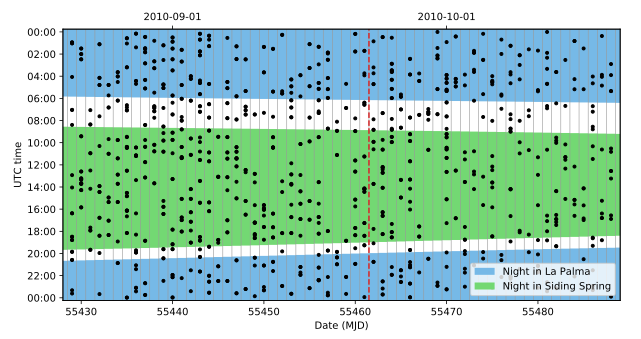
\includegraphics[width=\linewidth]{images/f2y_times.png}
\end{center}

\caption[Date and time distribution of events in the First Two Years sample]{Date and time distribution of events in the First Two Years sample \citep{First2Years}. The night periods are shown for La Palma and Siding Spring. The equinox is shown by the red dashed line. \rtxt{TODO --- Inkscapify}
}
\label{fig:f2y_times}
\end{figure}

Events were uniformly distributed across the sky, and are uniform in distance cubed. Although each source included distance information this was not taken into account in the simulations aside from determining the event strategy to use (all were well within the \SI{400}{\mega\parsec} definition for close neutron star events defined for GOTO-alert in \aref{sec:event_strategy}). Future simulations could use the distance to the event to estimate a light curve based on that of GW170817 and use it to predict how long each event would be visible for. As GW170817 only faded below \gls{goto}'s 20 mag limit after 2.5 days a 24 hour period is a reasonable amount of time to simulate.

The first stage of the simulations was to determine if the event source was going to be physically visible from the considered sites in the 24 hours after the event occurred. In order to save time it decided to not spend time running full fake pilot simulations for events which would never be observed, and therefore the simulation for that event was aborted early if no tiles that the source was located within were going to be visible. Each event was classified into four categories:

\begin{itemize}
    \item \textbf{Not visible --- too close to the Sun}. These events had sources that were too close to the Sun within the 24 hour period to observe. This was defined as being within \SI{42}{\degree} of the Sun at any point over the 24 hours (\SI{12}{\degree} from the definition of night time plus \SI{30}{\degree} from the horizon limit). This region corresponded to an area of the sky that would not be visible from any site on Earth using these observing parameters. This is a fixed fraction of the sky: 5280 sq deg or 13\% of the celestial sphere\footnote{The area of a circle with radius $r$ on the surface of a sphere with radius $R$ is $2\pi R^2(1-\cos(r))$. The radius of the celestial sphere $R=\SI{360}{\degree}/2\pi \approx \SI{57.3}{\degree}$.}.
    \item
    \item \textbf{Not visible --- below declination limit}. These event sources fall within the region of the sky that are never visible form a given site due to the limited declination range. For example, using the standard \SI{30}{\degree} horizon limit over the course of a year sa telescope on La Palma (latitude \SI{28}{\degree} N) can see a band of sky between \SI{+88}{\degree} and \SI{-32}{\degree} declination. Sources outside of this region (that are not already excluded due to being too close to the Sun) would therefore never be observable from the given site, but could be observed from other locations. At the equator this band covers 87\% of the sky, at latitudes of $\pm \SI{30}{\degree}$ 75\% of the sky is visible, falling to just 25\% at the poles\footnote{The area of a segment on a sphere between angles $\theta$ and $\phi$ is $2 \pi R^2 (\cos(\theta)-\cos(\phi))$}.
    \item
    \item \textbf{Not visible --- event time}. These event sources are outside of the hard Sun limit and within the visible declination range, but are still not observable during the given 24 hour period.

\end{itemize}


Timing and positions are pretty evenly spread (check paper).

Visibility: depends on sites, position of the Sun etc.

% ---------
\subsubsection{Selecting event tiles}

Selection is a small issue, some are just so far from the contours. Differs depending on the grid. See \autoref{sec:db_insert}.

% ---------
\subsubsection{Results of full pilot simulations}

How the simulations worked: real GOTO-alert commands, real database, real scheduler, fake pilot.

Results.

Analysis:
\begin{itemize}
    \item Different grids are different.
    \item Small gain from additional telescopes at the same site.
    \item Huge gain from multiple sites.
    \item Benefit from combining vs two independent.
\end{itemize}

Still to do:
\begin{itemize}
    \item weather
    \item SA?\@ Chile?
\end{itemize}

\end{colsection}

% ~~~~~~~~~~~~~~~~~~~~

\subsection{All-sky survey simulations}
\label{sec:allsky_sims}
\begin{colsection}

Simulate over a whole year.

Using the real scheduler takes a long time.

Light version is much easer, just selects based on altitude.

Get results for cadence, coverage, airmass?

Compare to real results over first 5 months, Feb-Jul (shame not 6 months).

\end{colsection}

% ~~~~~~~~~~~~~~~~~~~~

\end{colsection}

% ########################################
